\documentclass[crop,tikz]{standalone}%

\usepackage{../macro}

\usetikzlibrary{positioning}% To get more advances positioning options

\begin{document}

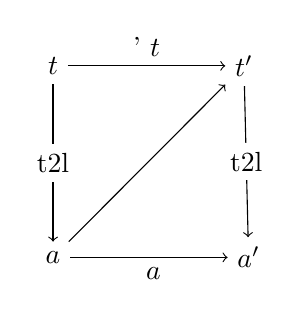
\begin{tikzpicture}[]
    \node (t1) at (0,0) {$t$};
    \node (t2) [right=2cm of t1]  {$t'$};
    \node (e1) [below=2cm of t1]  {$a$};
    \node (e2) [right=2cm of e1]  {$a'$};
    % letf to right arrows
    % \draw [->] (t1) -- (t2)node[pos=1,xshift=1pt,yshift=2pt]{*} node[midway, above]{\run'\ $t$};
    % \draw [->] (e1) -- (e2)node[pos=1,xshift=1pt,yshift=2pt]{*} node[midway, below]{\nur\ $a$};
    \draw [->] (t1) -- (t2) node[midway, above]{\run'\ $t$};
    \draw [->] (e1) -- (e2) node[midway, below]{\nur\ $a$};

    % up to down arrows
    \path [->] (t1) edge node[fill=white, anchor=center]{t2l} (e1);
    \path [->] (t2) edge node[fill=white, anchor=center]{t2l} (e2);

    % diagonal arrow
    % \path[->] (e1) edge node[fill=white, anchor=center, pos=0.5, rotate=45] {induction} (t2);
    \path[->] (e1) edge (t2);
\end{tikzpicture}


\end{document}
